\documentclass[conference]{acmsiggraph}

% http://en.wikibooks.org/wiki/LaTeX/Algorithms
\usepackage{algorithm2e}
% \usepackage{algpseudocode}

\usepackage{float}
\usepackage{caption}
\usepackage{amsmath}
\usepackage{url}
\usepackage{hyperref}

\newcommand\blfootnote[1]{%
  \begingroup
  \renewcommand\thefootnote{}\footnote{#1}%
  \addtocounter{footnote}{-1}%
  \endgroup
}

\TOGonlineid{45678}
\TOGvolume{0}
\TOGnumber{0}
\TOGarticleDOI{1111111.2222222}
\TOGprojectURL{}
\TOGvideoURL{}
\TOGdataURL{}
\TOGcodeURL{}

\title{Chronographer - Location History Visualization}


\author{Scott Todd\thanks{email: todds@rpi.edu}}
\pdfauthor{Scott Todd}

\keywords{Data Visualization, Geographic Data, Virtual Reality}

\begin{document}

\teaser{
    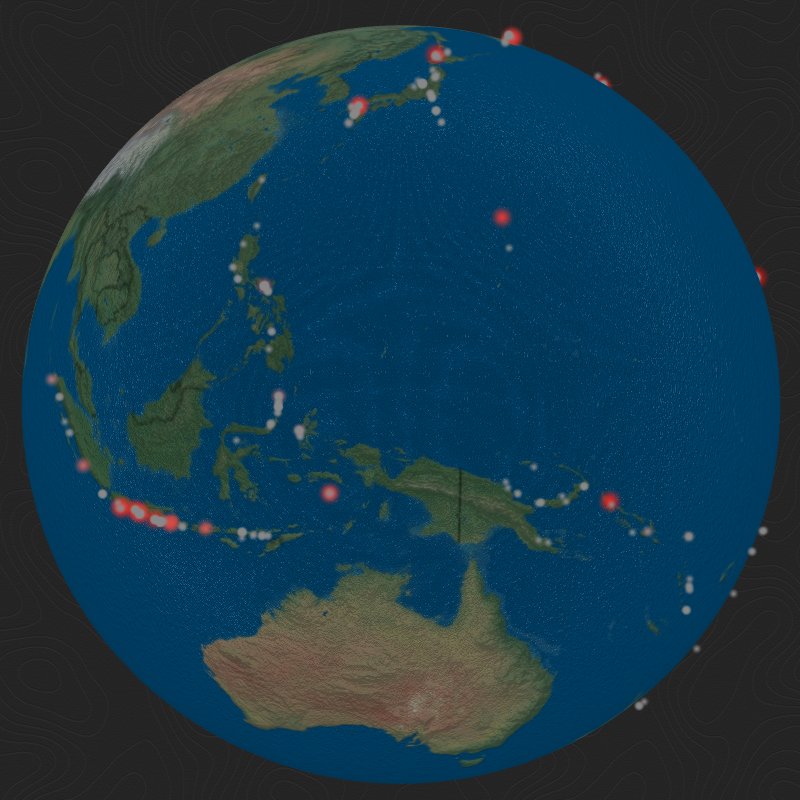
\includegraphics[height=180px]{images/chronographer.png}
    \captionsetup{hypcap=false}
    \caption{Visualizing volcanic eruptions.}
}

\maketitle


\begin{abstract}

I created a geographic location history visualization tool titled Chronographer
that explores virtual reality interaction as a data analysis aid. I used
three.js \cite{three.js}, the device orientation API
\cite{Mozilla:DeviceOrientation}, and the Google Cardboard
\cite{Google:Cardboard} viewer to construct this visualization, which is hosted
at \url{http://scotttodd.github.io/Chronographer/}. I visualized location
history data exported from my Google account using Google Takeout
\cite{Google:Takeout} as well as volcanic eruption data from NOAA
\cite{NOAA:Volcano}. I went through several design iterations and concluded that
this style of visualization is interesting but not currently effective as a
tool for learning from geographic data sets. I conducted informal user testing
partway through the project but did not perform a rigorous user study.

\end{abstract}

\keywordlist

\TOGlinkslist

%% Required for all content.
\blfootnote{Project Repository: https://github.com/ScottTodd/Chronographer}

\copyrightspace


\section{Introduction}

Geographic location history data sets combine spatial information which demands
context with chronological information which benefits greatly from interaction
or animation. Existing map-based tools present geographic data in an
understandable format but they each rely on a projection that introduces an
extra level of processing in order to relate the data to the physical world.
Virtual reality has been growing in popularity and technical maturity in recent
years and offers the opportunity to connect people to data in ways not possible
before. I wanted to test the utility of virtual reality in helping people
understand these data sets.

The representation of the time axis is also important for data analysis.
Several techniques have been researched in the past which handle user control
over the time axis differently.

Virtual reality devices such as the Oculus Rift and Sony's Project Morpheus are
currently in active development. Screen, positional tracking, and rendering
technologies have advanced to the point where immersive virtual reality is
nearly within reach for consumer-grade projects. The Google Cardboard takes this
a step further and leverages current generation smart phones, which are packed
with sensors and high resolution screens already, to deliver an affordable
virtual reality solution that hobbyists and consumers can easily use.

Virtual reality for web browsers is a recent extension of these new
technologies, so support and stability are both limited. The device orientation
API is experimental and has several shortcomings, but it may eventually be
replaced with official browser support through a technology currently being
named WebVR.


\subsection{Related Work}

\subsection{Technical References}

``What is Spatial History'' by Richard White \cite{White} details efforts to
chronicle history through data visualization, making sense of large data sets
through visual media, rather than through words alone as traditional history
textbooks do. He argues that spatial relations are established through movement
- movement of people, goods, and information. He discusses
``relational space'', where locations are closer at different points during a
day due to traffic and other relative, modern factors. He also concludes that
visualizations are a means of doing research and generating questions that may
have otherwise gone unasked, not a method to communicate findings discovered
through other means.

The DimpVis system \cite{10.1109/TVCG.2014.2346250} explores a novel method of
interacting with data points on two-dimensional plots with time as a third
axis. Where time is normally controlled by a slider, it allows for users to
drag points along hint paths to move through time in either direction.

\subsection{Further Inspiration}

GitHub user @theopolisme created a website that lets you visualize your Google
Location History using an interactive heatmap
\cite{location-history-visualizer}. In his visualization, data points from all
time values are compressed onto a single map which features zoom and pan
controls.

This blog post \cite{VR:BigData} argues that good data visualization tools
should consider human visual perception and give insight into the unknown, not
the already-understood. It explains how DARPA used the Oculus Rift to visualize
three-dimensional network simulations and how engineers at Caltech used virtual
worlds such as Second Life and the Unity3D game engine as data visualization
platforms.


\section{Development}

\subsection{Data}

The data returned through Google Takeout is in JSON form with a simple array
of [latitude, longitude, timestamp] triples.

\subsection{Initial Ideas}

I originally planned to build a two dimensional map interface that would blend
a set of data points across time ranges together. At this point, I was inspired
by @theopolisme's Location History Visualizer and had recently completed another
map-based visualization using d3.js \cite{D3.js}. Because of my familiarity with
d3.js and three.js, I hoped to combine the powerful WebGL rendering of three.js
with the convenient map projection and rendering of d3.js to visualize my own
location history. I had also been searching for a reason to experiment with the
Google Cardboard, so I worked that into my plans.

My basic visual design centered around displaying data points above a map and
using additive or alpha blending to show general regions where points were
focused. As the visualization time changed, data points would fade in and out.
I used a traditional slider to control the visualization time, which could be
set to play automatically or could be manually controlled via mouse or touch.
This initial design can be seen in Figure 2.

I used a particle system to represent data points, with each data point having
a single particle in the particle system to represent it. These particles would
change their display properties based on the difference between the
visualization time and their data point's time through computations in a set
of custom vertex and fragment shaders (see Algorithm 1).

\RestyleAlgo{boxruled}
\begin{algorithm}
\DontPrintSemicolon
\caption{Data Point Rendering}
    \KwData{$visualizationTime$, $minTime$, $maxTime$, $highlightPercent$}
    \ForEach{particle} {
        \KwData{$particleTime$, $latitude$, $longitude$}
        \begin{enumerate}
            \item Position in object space based on $latitude$ and \\
                $longitude$
            \item Compute $visPercent$ as the percentage that
                $visualizationTime$ is from $minTime$ to $maxTime$
            \item Compute $particlePercent$ as the percentage that
                $particleTIme$ is from $minTime$ to $maxTime$
            \item Compute $percentDifference$ and scale by $highlightPercent$
            \item Interpolate HSV color, size, and alpha using this scaled
                percentage
        \end{enumerate}
    }
\end{algorithm}

\begin{figure}[b]
  \centering
  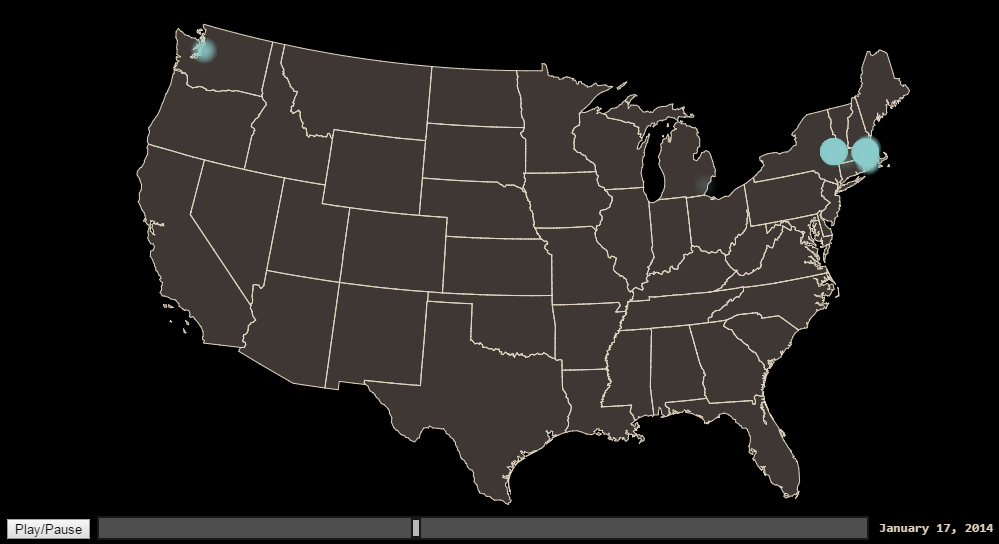
\includegraphics[width=3.4in]{images/initial_us_map}
  \caption{Initial map of the USA with data point particles. Note the slider at
           the bottom of the screen.}
\end{figure}

\subsection{First Extensions}

After producing a working 2D implementation of my basic idea, I experimented
with other projections (Figures 3 and 4), eventually aiming for a spherical
projection that would have potential as an effective virtual reality view.

\begin{figure}
  \centering
  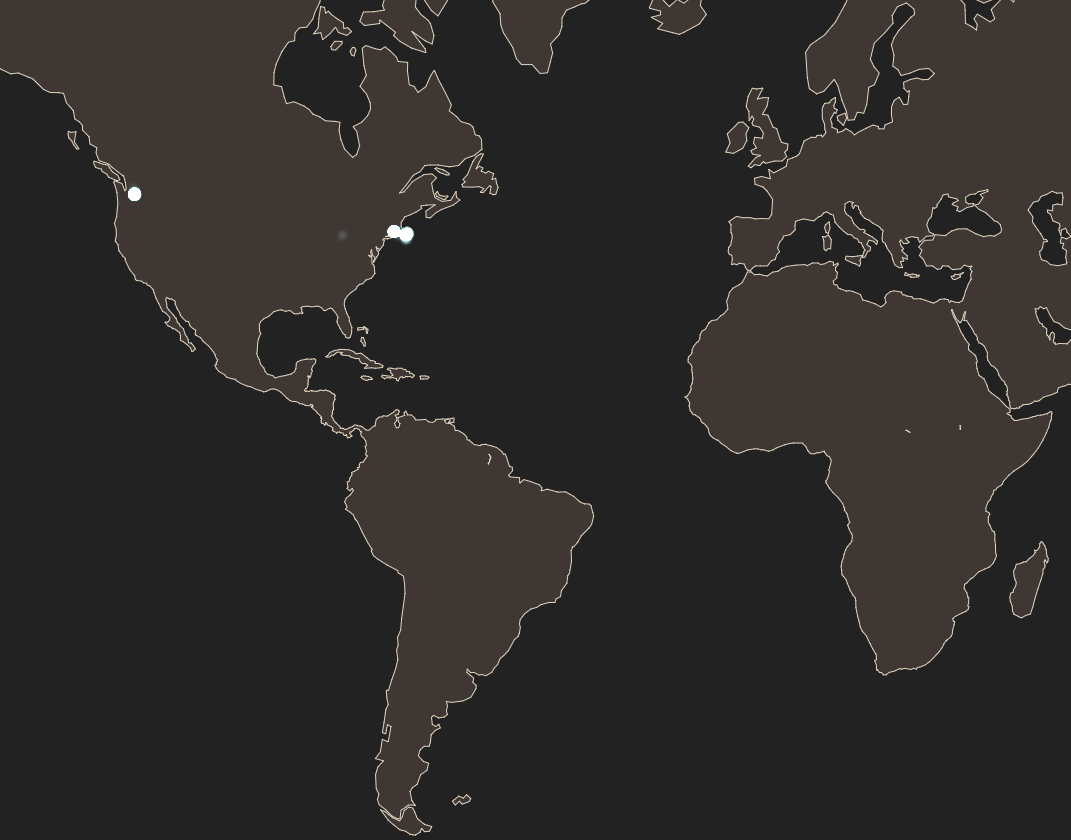
\includegraphics[width=3.0in]{images/mercator_projection_with_particles}
  \caption{Mercator projection with data point particles.}
\end{figure}

\begin{figure}
  \centering
  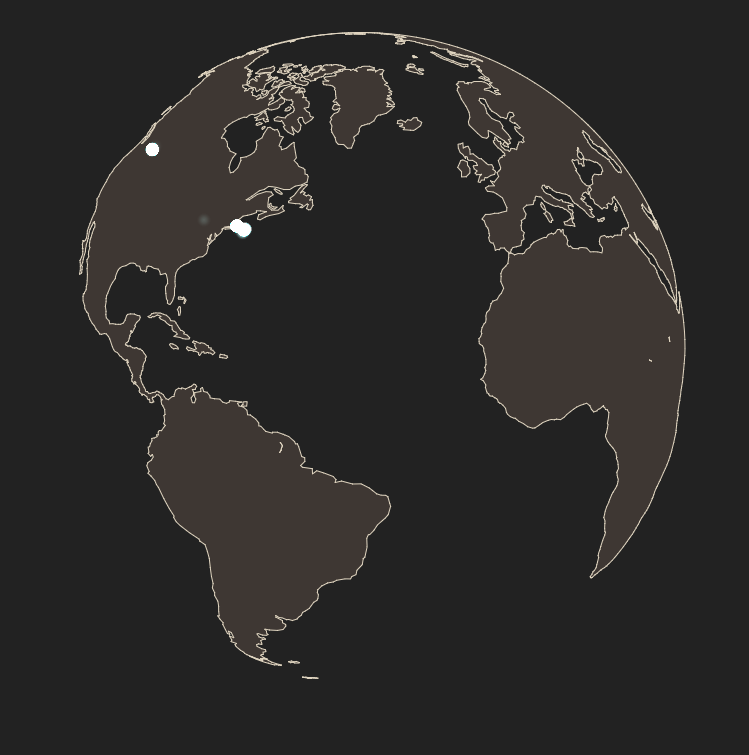
\includegraphics[width=3.0in]{images/orthographic_projection_with_particles}
  \caption{Orthographic projection with data point particles.}
\end{figure}

Up until this point, I had been combining d3.js and three.js and used an awkward
bridge between them to reliably communicate the projection and viewport
information needed to render both a map and a particle system on the same
screen (see Algorithm 2). I realized that if I switched entirely to a spherical
projection, I could render the map using three.js rather than with d3.js,
removing the need to operate through that additional level of abstraction.

\RestyleAlgo{boxruled}
\begin{algorithm}
\DontPrintSemicolon
\caption{Initial Data Point Positioning}
    At load time : \ForEach{data point} {
        Create a particle in the particle system, storing latitude and longitude
    }
    At run time : \ForEach{frame} {
        \ForEach{particle} {
            \begin{enumerate}
                \item Convert from latitude/longitude to screen-space \\
                    {[}x, y{]} using d3.geo.projection
                \item Convert from screen-space {[}x, y{]} to three.js \\
                    world-space {[}x, y, z{]} using \\
                    THREE.Projector.unprojectVector
                \item Update {[}x, y, z{]} vertex position for this particle
            \end{enumerate}
        }
        Render all particles using a custom vertex and fragment \\ shader
    }
\end{algorithm}

\subsection{Final Details}


\section{Feedback}

\section{Results}

Results.


\section{Limitations and Future Work}

Limitations and future work.


\section{Conclusions}

Conclusions.

\section{Acknowledgments}

Acknowledgments.

\bibliographystyle{acmsiggraph}
\bibliography{chronographer}
\end{document}
